% $Id$
%

\section{HTML5}


%% LICENCIA DE REDISTRIBUCION DE LAS TRANSPAS
\frame{
~
\vspace{1cm}

\begin{flushright}
\copyright Mark Pilgrim \\
\copyright Gregorio Robles - Universidad Rey Juan Carlos \\
\vspace{1cm}

Algunos derechos reservados. Este artículo se distribuye bajo
la licencia ``Reconocimiento 3.0 España'' de Creative Commons,
disponible en \\
{\small \url{http://creativecommons.org/licenses/by/3.0/es/deed.es}}
\vspace{1cm}

Este documento se basa en el libro ''Dive into HTML5'' \\
disponible en http://diveintohtml5.info/
\end{flushright}
}


%%---------------------------------------------------------------
%%---------------------------------------------------------------

\subsection{5 cosas sobre HTML5}

%%---------------------------------------------------------------

\begin{frame}
\frametitle{1. No es una única cosa grande}

\begin{itemize}
  \item HTML5 es una colección de funcionalidades
  \item No hace falta buscar soporte completo, pero sí de las funcionalidades concretas
  \item HTML5 especifica también cómo interactuar con JavaScript y DOM
\end{itemize}

\end{frame}

%%---------------------------------------------------------------

\begin{frame}
\frametitle{2. No hace falta tirar nada}

\begin{itemize}
  \item Se basa en HTML4
  \item Si una web funcionaba con HTML4, funcionará con HTML5
  \item HTML5 extiende HTML4 
  \item Los navegadores antiguos tratarán muchos elementos HTML5 como si no existieran
\end{itemize}

\end{frame}

%%---------------------------------------------------------------

\begin{frame}[fragile]
\frametitle{3. Es fácil empezar}

\begin{itemize}
  \item Cambiar a HTML5 es sencillo
  \item En realidad, sólo hay que cambiar el DOCTYPE:
\begin{verbatim}
<!DOCTYPE html>
\end{verbatim}
  \item Los elementos obsoletos de HTML4 todavía se verán en HTML5
\end{itemize}

\end{frame}

%%---------------------------------------------------------------

\begin{frame}
\frametitle{4. Ya funciona (en líneas generales)}

\begin{itemize}
  \item Los navegadores están haciendo un gran esfuerzo por incluir HTML5
  \item Mientras tanto, tendremos que estar atentos a la compatibilidad de los mismos
  \item Todavía no está totalmente estandarizado
  \item Hasta 2020 no se espera soporte completo
\end{itemize}

\end{frame}

%%---------------------------------------------------------------

\begin{frame}
\frametitle{5. Está aquí para quedarse}

\begin{itemize}
  \item Reemplaza otras tecnologías: Flash
  \item Sigue la tendencia de que todo va a la nube
  \item Sigue la tendencia de la ubicuidad
\end{itemize}

\end{frame}


%%---------------------------------------------------------------
%%---------------------------------------------------------------

\subsection{Algunos elementos HTML5}
%%---------------------------------------------------------------

\begin{frame}[fragile]
\frametitle{DOCTYPE}

\begin{itemize}
  \item Hasta ahora había diferentes modos:
  \begin{itemize}
    \item Quirks Mode
    \item Standards Mode
    \item Almost Standards Mode
  \end{itemize}
  \item En HTML5, sólo hace falta:
\begin{verbatim}
<!DOCTYPE html>
\end{verbatim}
\end{itemize}

\end{frame}

%%---------------------------------------------------------------

\begin{frame}[fragile]
\frametitle{El Elemento raíz}

\begin{itemize}
  \item Antes:
\begin{verbatim}
<html xmlns="http://www.w3.org/1999/xhtml"
      lang="en"
      xml:lang="en">
\end{verbatim}
  \item Ahora:
\begin{verbatim}
<html lang="en">
\end{verbatim}
\end{itemize}

\end{frame}

%%---------------------------------------------------------------

\begin{frame}[fragile]
\frametitle{Codificación de caracteres}

\begin{itemize}
  \item Si podemos, envíamos cabecera:
\begin{verbatim}
Content-Type: text/html; charset="utf-8"
\end{verbatim}
  \item Si no se puede, en HTML5:
\begin{verbatim}
<meta charset="utf-8" />
\end{verbatim}

\end{itemize}

\end{frame}

%%---------------------------------------------------------------

\begin{frame}
\frametitle{Elementos semánticos}

\begin{itemize}
  \item $<section>$
  \item $<nav>$
  \item $<article>$
  \item $<aside>$
  \item $<hgroup>$
  \item $<header>$
  \item $<footer>$
  \item $<time>$
  \item $<mark>$
\end{itemize}

\end{frame}

%%---------------------------------------------------------------

\begin{frame}[fragile]
\frametitle{¿Cómo muestran los navegadores elementos desconocidos?}

\begin{itemize}
  \item Las etiquetas desconocidas se muestran como si fueran ''inline''
  \item Regla CSS para cambiar el comportamiento (p.ej., en Bootstrap):
\begin{verbatim}
article,aside,details,figcaption,figure,
footer,header,hgroup,menu,nav,section {
    display:block;
}
\end{verbatim}

Las versiones antiguas de Internet Explorer son especialmente ''particulares''.

\end{itemize}

\end{frame}


%%---------------------------------------------------------------

\begin{frame}
\frametitle{Relaciones}

\begin{itemize}
  \item Hoja de estilo: rel=''stylesheet''
  \item Feed: rel=''alternate''
  \item Emoticono: rel=''shortcut icon''
  \item Serie de páginas:  rel=''start'', rel=''prev'', rel=''next''
  \item ...
\end{itemize}

\end{frame}


%%---------------------------------------------------------------
%%---------------------------------------------------------------

\section{Canvas}
%%---------------------------------------------------------------

\begin{frame}[fragile]
\frametitle{La etiqueta canvas}

\begin{itemize}
  \item Elemento canvas
  \item Se ha de especificar un tamaño (width y height)
  \item Requiere un id para poder manipularla
  \item El canvas siempre empieza vacío
  \item Si el navegador no lo entiende, muestra el texto entre las etiquetas.
  \item También es usado por WebGL para pintar gráficos 3D optimizados por hardware.
\end{itemize}

\begin{verbatim}
  <canvas id="a" width="300" height="225">
    Your browser does not support HTML5 canvas.
  </canvas>
\end{verbatim}

\end{frame}

%%---------------------------------------------------------------

\begin{frame}[fragile]
\frametitle{Pintemos algo}

\begin{verbatim}
function draw_b() {
  var b_canvas = document.getElementById("b");
  var b_context = b_canvas.getContext("2d");
  b_context.fillRect(50, 25, 150, 100);
}
\end{verbatim}

\end{frame}

%%---------------------------------------------------------------

\begin{frame}
\frametitle{Algunas cuestiones a la hora de pintar}

\begin{itemize}
  \item La propiedad \emph{fillStyle} puede ser cualquier color CSS (también un patrón o un gradiente). Por defecto, es negro.
  \item fillRect(x, y, width, height) pinta un rectángulo relleno (con el color de \emph{fillStyle}).
  \item La propiedad \emph{strokeStyle} es como \emph{fillStyle} pero para líneas.
  \item strokeRect(x, y, width, height) pinta un rectángulo con el estilo de \emph{strokeStyle}.
  \item clearRect(x, y, width, height) borra los píxeles del rectángulo especificado.
\end{itemize}

\end{frame}

%%---------------------------------------------------------------

\begin{frame}
\frametitle{Sobre las coordenadas}

\begin{itemize}
  \item La coordenada (0,0) está en la esquina superior izquierda del canvas
  \item El eje X crece hacia la derecha
  \item El eje Y crece hacia abajo (!!)
\end{itemize}

\end{frame}

%%---------------------------------------------------------------

\begin{frame}
\frametitle{Caminos}

\begin{itemize}
  \item beginPath(): empieza un nuevo camino
  \item moveTo(x, y): sitúa el lápiz en la coordenada especificada.
  \item lineTo(x, y): pinta una línea hasta la coordenada especificada.
  \item stroke(): dibuja (con el estilo de \emph{strokeStyle}).
  \item arc(x, y, radio, angulo\_comienzo, angulo\_final, direccion);
  \begin{itemize}
    \item angulo\_comienzo y angulo\_final pueden ser p.ej. Math.PI * 2
    \item direccion: false si en el sentido del reloj
  \end{itemize}
\end{itemize}

\end{frame}


%%---------------------------------------------------------------

\begin{frame}
\frametitle{Texto}

\begin{itemize}
  \item font: como \emph{font} de CSS.
  \item textAlign: como el \emph{text-align} de CSS.
  \item textBaseLine: top, hanging, middle, alphabetic, ideographic, o bottom.
  \item fillText(''texto'', x, y): introduce ''texto'' en la posición (x, y).
\end{itemize}

\end{frame}

%%---------------------------------------------------------------

%\begin{frame}
%\frametitle{Ejercicio: Pintemos un diagrama de coordenadas}
%
%\begin{center}
%\begin{figure}[p]
%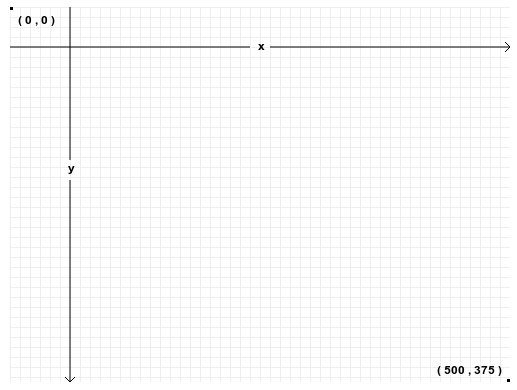
\includegraphics[width=0.8\textwidth]{figs/diagramacoordenadas.png}
%\end{figure}
%\end{center}
%
%\end{frame}


%%---------------------------------------------------------------

\begin{frame}
\frametitle{Imágenes (I)}

\begin{itemize}
  \item drawImage(image, dx, dy): toma la imagen ''image'' y la pinta en el canvas. Las coordenadas dx y dy dan la esquina superior izquierda de la imagen.
  \item drawImage(image, dx, dy, dw, dh): toma la imagen ''image'' y la pinta en el canvas. Las coordenadas dx y dy dan la esquina superior izquierda de la imagen escalándola a una anchura dw y a una altura dh.
  \item drawImage(image, sx, sy, sw, sh, dx, dy, dw, dh): toma la imagen ''image'' y la introduce en el rectángulo (sx, sy, sw, sh), escalándola a las dimensiones (dw, dh), y la pinta en las coordenadas (dx, dy). Véase la siguiente transparencia.
\end{itemize}

\end{frame}

%%---------------------------------------------------------------

\begin{frame}
\frametitle{Imágenes (y II)}

\begin{center}
\begin{figure}[p]
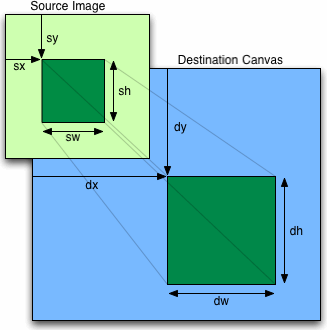
\includegraphics[width=0.6\textwidth]{figs/drawImage.png}
\end{figure}
\end{center}

\end{frame}


%%---------------------------------------------------------------

\begin{frame}
\frametitle{Referencias sobre Canvas}

\begin{itemize}
  \item Canvas HTML element: \\ {\footnotesize \url{https://developer.mozilla.org/en-US/docs/Web/HTML/Element/canvas}}
  \item Canvas API: \\ {\footnotesize \url{https://developer.mozilla.org/en-US/docs/Web/API/Canvas_API}}
\end{itemize}

\end{frame}

%%---------------------------------------------------------------
%%---------------------------------------------------------------

\section{Local Storage}

%%---------------------------------------------------------------

\begin{frame}
\frametitle{Buscando un espacio para guardar en local}

¿Y por qué no las cookies?

\begin{enumerate}
  \item Las cookies se incluyen en cada petición HTTP, ralentizando una aplicación al enviarse una y otra vez
  \item Las cookies se incluyen en cada petición HTTP, enviando datos de manera no cifrada (a menos de que toda la aplicación se sirva sobre SSL)
  \item Las cookies están limitadas a 4KB de datos - suficiente para ralentizar la conexión (véase punto 1), pero no lo suficiente para ser muy útiles
\end{enumerate}

\end{frame}

%%---------------------------------------------------------------

\begin{frame}
\frametitle{HTML5 storage (Web storage)}

\begin{itemize}
  \item Es una manera de guardar parejas llave/valor de manera local, en el navegador cliente
  \item Estos datos persisten aún cuando cerremos el navegador
  \item Estos datos no se transmiten al servidor, a menos de que se pidan de manera explícita
  \item Es un mecanismo implementado de manera nativa en navegadores web, evitando tener que utilizar plug-ins y otras extensiones/trucos.
\end{itemize}

\end{frame}

%%---------------------------------------------------------------

\begin{frame}[fragile]
\frametitle{Accediendo al almacenamiento local}

La intefaz:

\begin{verbatim}
interface Storage {
  getter any getItem(in DOMString key);
  setter creator void setItem(in DOMString key, in any data);
};
\end{verbatim}

Ejemplo de uso:
\begin{verbatim}
var foo = localStorage.getItem("bar");
localStorage.setItem("bar", foo);
\end{verbatim}

También vale:
\begin{verbatim}
var foo = localStorage.bar;
localStorage.bar = foo;
\end{verbatim}


También valdría (p.ej., para iterar con un \emph{for}):
\begin{verbatim}
var foo = localStorage["bar"];
localStorage["bar"] = foo;
\end{verbatim}


\end{frame}

%%---------------------------------------------------------------

\begin{frame}[fragile]
\frametitle{Borrando e iterando el almacenamiento local}

Interfaz de borrado:

\begin{verbatim}
interface Storage {
  deleter void removeItem(in DOMString key);
  void clear();
};
\end{verbatim}

Interfaz de iteración:

\begin{verbatim}
interface Storage {
  readonly attribute unsigned long length;
  getter DOMString key(in unsigned long index);
};

\end{verbatim}


\end{frame}


%%---------------------------------------------------------------

\begin{frame}
\frametitle{Referencias sobre Local Storage}

\begin{itemize}
  \item Local Storage API: \\ {\footnotesize \url{https://developer.mozilla.org/en-US/docs/Web/API/Window/localStorage}}
  \item Ejemplos de uso: \\ {\footnotesize \url{https://developer.mozilla.org/en-US/docs/Web/API/Web_Storage_API/Using_the_Web_Storage_API}}
\end{itemize}

\end{frame}


%%---------------------------------------------------------------
%%---------------------------------------------------------------

\section{Detección de funcionalidad HTML5}

%%---------------------------------------------------------------

\begin{frame}
\frametitle{Técnicas de detección de características HTML5}

Dependiendo de la característica, hay que:

\begin{enumerate}
  \item Comprobar si existe una propiedad en un objeto global (como window o navigator). P.ej. geolocalización.
  \item  Crear un elemento y entonces comprobar si existe una propiedad específica en ese elemento. P.ej. soporte para canvas.
  \item Crear un elemento, comprobor si existe un método específico en ese elemento y entonces llamar al método y comprobar el valor de retorno. P.ej. comprobar formatos de vídeo soportados
  \item Crear un elemento, poner un valor a una propiedad, y comprobar si la propiedad ha retenido ese valor. P.ej. comprobar los tipos de $<input>$ soportados
\end{enumerate}

... o simplemente se puede utilizar la biblioteca JavaScript Modernizr (que te abstrae de todo lo anterior)


\end{frame}

%%---------------------------------------------------------------

\begin{frame}[fragile]
\frametitle{Modernizr}

\begin{verbatim}
if (Modernizr.ELEMENT) {
  // let's go!
} else {
  // no native ELEMENT support available :(. 
  // Maybe try a fallback
}
\end{verbatim}

donde \emph{ELEMENT} puede ser: canvas, canvastext, video, video.webm, video.ogg, video.h264, localstorage, webworkers, applicationcache, geolocation, input.autofocus, history...

\end{frame}



\begin{frame}
\frametitle{Polyfills}

\begin{itemize}
  \item Si una característica HTML5 no está soportada por el navegador, podemos
  usar \emph{polyfills}
  \item Los \emph{polyfills} son bibliotecas, módulos externos que ofrecen funcionalidad
  parecida a los que HTML5 ofrece de forma nativa.
  \item Puede haber varios \emph{polyfills} para cada característica.
  \item Se tienen que evaluar y probar de manera independiente.
  \item Para probarlo, hace falta un navegador que no implemente HTML5 (p.ej. Konqueror para algunas funcionalidades)
\end{itemize}

\end{frame}

%%---------------------------------------------------------------
%%---------------------------------------------------------------

\section{Geolocalización}


%%---------------------------------------------------------------

\begin{frame}[fragile]
\frametitle{Un ejemplo de geolocalización}

\begin{verbatim}
function get_location() {
  if (Modernizr.geolocation) {
    navigator.geolocation.getCurrentPosition(show_map);
  } else {
    // no native support; maybe try a fallback?
  }
}
\end{verbatim}

Geolocalización es opt-in para el usuario. Este código ofrece un menú donde
puede compartir su geolocalización o no.

\end{frame}

%%---------------------------------------------------------------

\begin{frame}[fragile]
\frametitle{Sigamos con el ejemplo}

\begin{verbatim}
function show_map(position) {
  var latitude = position.coords.latitude;
  var longitude = position.coords.longitude;
  // let's show a map or do something interesting!
}
\end{verbatim}

La función \emph{callback} se llamará con un único parámetro: un objeto con dos
propiedades: \emph{coords} y \emph{timestamp}

\end{frame}

%%---------------------------------------------------------------

\begin{frame}
\frametitle{El objeto posición}

\begin{footnotesize}
\begin{tabular}{ l c l }
Propiedad & Tipo & Nota \\
\hline
coords.latitude	& double	& decimal degrees \\
coords.longitude & double	& decimal degrees \\
coords.altitude	& double or null	& meters above reference ellipsoid \\
coords.accuracy	& double	& meters \\
coords.altitudeAccuracy	& double or null	& meters \\
coords.heading	& double or null	& degrees clockwise from true north \\
coords.speed	& double or null	& meters/second \\
timestamp	& DOMTimeStamp	& like a Date() object \\
\end{tabular}
\end{footnotesize}

\end{frame}


%%---------------------------------------------------------------
%%---------------------------------------------------------------

\section{Web Workers}

%%---------------------------------------------------------------

\begin{frame}
\frametitle{¿Qué son?}

\begin{itemize}
  \item Scripts en JavaScript que se ejecutan en el \emph{background}
  \item Por tanto, no bloquean la página (los navegadores suelen ser de un único hilo)
  \item Son parecidos a los \emph{threads} (¡pero no comparten memoria!)
  \item Son relativamente pesados... sólo deberían utilizarse si van a realizar
tareas pesadas que hagan que el coste de iniciar uno (en memoria y en procesamiento)
valga la pena
  \item Los Web Workers no tienen acceso al DOM, se comunican con el programa principal mediante
envío de mensajes.
\end{itemize}

\end{frame}


%%---------------------------------------------------------------

\begin{frame}[fragile]
\frametitle{¿Cómo se lanzan?}

\begin{enumerate}

  \item Se instancia un objeto Worker, cuyo parámetro es una URL con el código JavaScript
  La URL tiene las mismas limitaciones de seguridad que JavaScript.
  Se puede empotrar en código JavaScript en la misma página HTML, pero entonces hay que
crear un objeto URL.

  \begin{verbatim}
var worker = new Worker("worker.js");
  \end{verbatim}

  \item Se pasa un mensaje al Worker.
  Normalmente este mensaje estará en formato JSON (con \emph{stringify}).

  \begin{verbatim}
worker.postMessage("Hello World!");
  \end{verbatim}
\end{enumerate}

\end{frame}


%%---------------------------------------------------------------

\begin{frame}[fragile]
\frametitle{¿Cómo se lanzan? (y II)}

\begin{enumerate}
  \setcounter{enumi}{2}

  \item En caso de recibir un mensaje de respuesta, se captura el evento y se hace lo que queramos con los datos que
recibidos (nota: generalmente recibiremos un JSON, al que se le pasa \emph{parse}):
  \begin{verbatim}
worker.onmessage = function(event) {
    console.log("Hemos recibido " + event.data);
    hacemosAlgo();
}
  \end{verbatim}

  \item Se da por cerrado el Worker (cuidado, ¡orientación a eventos!):
  \begin{verbatim}
worker.terminate();
  \end{verbatim}
\end{enumerate}

\end{frame}

%%---------------------------------------------------------------

\begin{frame}[fragile]
\frametitle{¿Cómo se ejecutan?}

\begin{itemize}
  \item El código del Worker estará en un fichero JavaScript separado (p.ej., \texttt{worker.js})
  \item Utiliza la misma interfaz de comunicación, con la salvedad de que en vez de realizarse sobre el objeto tipo \texttt{Worker} lo hace sobre sí mismo, con \emph{self}.
  \item Recuerda: no puede acceder al DOM
  \item Puede enviar varios mensajes, no tiene por qué ser un único
  \item Ejemplo de código de un \texttt{Workder} (en su fichero \emph{.js}):
\end{itemize}

\begin{verbatim}
self.onmessage = function(event) {
    console.log("He recibido " + event.data);
    salida = hacemosAlgo();
    self.postMessage("Te devuelvo " + salida)
}
\end{verbatim}

\end{frame}


%%---------------------------------------------------------------
%%---------------------------------------------------------------

\section{History API}

%%---------------------------------------------------------------

\begin{frame}
\frametitle{¿Qué es la History API?}


\begin{itemize}
  \item El objeto \texttt{window} del DOM proporciona acceso al historial del browser a través del objeto \texttt{history}
  \item Tendremos métodos y propoiedades que nos permitan avanzar y retroceder a través del historial (esto lo hemos podido hacer desde (casi) siempre)
  \item Podemos manipular el contenido del historial (¡nuevo en HTML5!)
\end{itemize}

\end{frame}

%%---------------------------------------------------------------

\begin{frame}
\frametitle{Moviéndonos en el historial}


\begin{itemize}
  \item Hacia atrás: window.history.back();
  \item Hacia adelante: window.history.forward();
  \item A un punto específico del historial: window.history.go(-2);
  \item Longitudo de la pila: window.history.length;
\end{itemize}

\end{frame}

%%---------------------------------------------------------------

\begin{frame}[fragile]
\frametitle{Manipulando el historial}


\begin{itemize}
  \item Añadir entradas en el historial: history.pushState();
\begin{verbatim}
var stateObj = { foo: "bar" };  
   // puede ser cualquier cosa que puedas pasar a JSON.stringify.
history.pushState(stateObj, "titulo pagina", 
       "introducida.html");
\end{verbatim}
  \item Modificar entradas en el historial: history.replaceState();
\begin{verbatim}
var stateObj = { foo: "bar" };
history.replaceState(stateObj, "titulo pagina", 
       "nueva.html");
\end{verbatim}
  \item Evento \texttt{popstate}: se lanza cada vez que la entrada al historial cambia.  la propiedad state del evento popstate contiene una copia del historial de entradas del objeto estado.
\end{itemize}

\end{frame}



%%---------------------------------------------------------------
%%---------------------------------------------------------------

%\section{Navegación Off-line: Service Workers}

%%---------------------------------------------------------------

%\begin{frame}
%\frametitle{Funcionamiento básico}

%\begin{itemize}
%  \item navigator.onLine es una propiedad que mantiene un valor true (online) / false (offline)
%  \item Esta propiedad se actualiza siempre que el usuario cambia a ``Modo sin conexión'' seleccionando el elemento de menú correspondiente (Archivo -> Trabajar sin conexión en Firefox).
%  \item 
%\end{itemize}

%(hay un flag en el DOM que indica si estamos on-line u off-line) \\
%(ojo: hay una manera antigua, app-caché, con un manifest que está \emph{deprecated})


%\end{frame}

%%---------------------------------------------------------------

%\begin{frame}[fragile]
%\frametitle{}
%
%\end{frame}

%%---------------------------------------------------------------

%\begin{frame}
%\frametitle{Referencias sobre Navegación off-line}

%\begin{itemize}
%  \item : \\ {\footnotesize \url{}}
%  \item : \\ {\footnotesize \url{}}
%\end{itemize}


%%---------------------------------------------------------------
%%---------------------------------------------------------------

\section{WebSocket}

%%---------------------------------------------------------------

\begin{frame}
\frametitle{¿Qué son los WebSockets?}

\begin{itemize}
  \item Protocolo que permite tener comunicación full-duplex sobre TCP (RFC 6455)
  \item Usa el puerto 80 (bueno para evitar firewalls)
  \item Es independiente de HTTP - el handshake es interpretado por los servidores como una petición \emph{Upgrade}
  \item Permite que el servidor envíe contenido al navegador sin que éste la haya solicitado
  \item Antes de la estandarización por el W3C, la solución pasaba por tecnologías como Comet
\end{itemize}

\end{frame}


%%---------------------------------------------------------------

\begin{frame}[fragile]
\frametitle{El \emph{handshake} con WebSockets}

{\bf Petición del cliente:}

\begin{verbatim}
GET /chat HTTP/1.1
Host: server.example.com
Upgrade: websocket
Connection: Upgrade
Sec-WebSocket-Key: x3JJHMbDL1EzLkh9GBhXDw==
Sec-WebSocket-Protocol: chat, superchat
Sec-WebSocket-Version: 13
Origin: http://example.com
\end{verbatim}

{\bf Respuesta del servidor:}

\begin{verbatim}
HTTP/1.1 101 Switching Protocols
Upgrade: websocket
Connection: Upgrade
Sec-WebSocket-Accept: HSmrc0sMlYUkAGmm5OPpG2HaGWk=
Sec-WebSocket-Protocol: chat
\end{verbatim}

\end{frame}


%%---------------------------------------------------------------

\begin{frame}[fragile]
\frametitle{Utilizando WebSockets}

\begin{enumerate}
  \item Instanciando un objeto WebSocket (nótese que la URL empieza por 'ws'; también existe conexión segura mediante el uso de 'wss'):
\begin{verbatim}
var connection = new WebSocket('ws://gsyc.es/echo');
\end{verbatim}

  \item Enviamos datos al servidor (lo suyo sería enviar JSON, pero podemos enviar también otras cosas, como Blob o ArrayBuffer):
\begin{verbatim}
connection.onopen = function () {
  connection.send('Ping'); 
};
\end{verbatim}

\end{enumerate}

\end{frame}


%%---------------------------------------------------------------

\begin{frame}[fragile]
\frametitle{Utilizando WebSockets (y II)}

\begin{enumerate}
  \setcounter{enumi}{2}

  \item Podemos mirar si hay errores:
\begin{verbatim}
connection.onerror = function (error) {
  console.log('Error en el WebSocket: ' + error);
};
\end{verbatim}

  \item Recibimos del servidor (generalmente serán JSON, pero se pueden recibir otras cosas, como Blob o ArrayBuffer):
\begin{verbatim}
connection.onmessage = function (e) {
  console.log('Server: ' + e.data);
};
\end{verbatim}

\end{enumerate}

\end{frame}


%%---------------------------------------------------------------

\begin{frame}
\frametitle{Implementaciones en el servidor}

\begin{itemize}
  \item Node.js
  \begin{itemize}
    \item Socket.IO
    \item WebSocket-Node
    \item ws
  \end{itemize}
  \item Python
  \begin{itemize}
    \item pywebsocket
    \item Tornado
  \end{itemize}
  \item Java
  \begin{itemize}
    \item Jetty
  \end{itemize}
  \item Ruby
  \begin{itemize}
    \item EventMachine
  \end{itemize}
\end{itemize}
\end{frame}


